\section{Mechanistic Changes after Repair}\label{app:postrepair}
\subsection{Paired measurements on unchanged context}
The mechanism-guided repair uses learned head adaptation and fixed native-projection restoration rather than the diagnostic mass or pattern replacements. We compare the native model and the seed-42 adapted/restored model on unchanged full-context inputs, using the frozen selected head identities. Neither the diagnostic bridge annotation nor a direct-query donor is used by the deployed repair policy.

\textbf{Paragraph access.} We join the native and adapted-state readout feature archives on canonical composed-question and source IDs, checking paragraph order, prompt length, paragraph token geometry and head identities. The selected-head average of paragraph attention mass is measured over question-token rows. The test set contains 1,000 sources per model; a fixed subset of 234/236/243 sources has correct native constituents but an incorrect native composition. Table~\ref{tab:postrepair_routing} reports paired changes on both populations. Intervals are 95\% source-bootstrap intervals with 10,000 draws.

\begin{table}[!ht]
\centering
\caption{\textbf{Paragraph access after adaptation and restoration.} Means are percentages; differences and 95\% intervals are in percentage points. The native failure subset is fixed before comparison.}
\label{tab:postrepair_routing}
\small
\begin{tabular}{llrrrr}
\toprule
Model & Population & $n$ & Paragraph & Native $\to$ Adapted & Change [95\% CI] \\
\midrule
Qwen3-4B & Test & 1000 & Root & 30.63 $\to$ 29.54 & $-1.09\ [-1.28,-0.90]$ \\
 & & & Bridge & 8.14 $\to$ 14.18 & $+6.04\ [5.80,6.28]$ \\
 & Fixed failures & 234 & Root & 31.02 $\to$ 29.97 & $-1.06\ [-1.43,-0.67]$ \\
 & & & Bridge & 7.63 $\to$ 12.99 & $+5.36\ [4.87,5.87]$ \\
\midrule
Qwen3-8B & Test & 1000 & Root & 31.56 $\to$ 31.13 & $-0.43\ [-0.55,-0.32]$ \\
 & & & Bridge & 8.96 $\to$ 13.29 & $+4.33\ [4.17,4.50]$ \\
 & Fixed failures & 236 & Root & 32.58 $\to$ 32.19 & $-0.39\ [-0.63,-0.14]$ \\
 & & & Bridge & 8.18 $\to$ 11.88 & $+3.71\ [3.40,4.02]$ \\
\midrule
Llama-3.1-8B & Test & 1000 & Root & 25.33 $\to$ 23.03 & $-2.29\ [-2.48,-2.11]$ \\
 & & & Bridge & 8.84 $\to$ 15.81 & $+6.97\ [6.72,7.22]$ \\
 & Fixed failures & 243 & Root & 26.32 $\to$ 24.32 & $-1.99\ [-2.37,-1.61]$ \\
 & & & Bridge & 7.38 $\to$ 13.84 & $+6.46\ [5.93,7.00]$ \\
\bottomrule
\end{tabular}
\end{table}

\textbf{Relation reading.} We reuse the 25 shared-context discovery quadruplets in the factorized intervention experiment. Each composed receiver has two direct questions naming the same bridge entity but requesting different relations. For each model we run the native composed query, its direct same-relation query, its direct other-relation query, and the adapted/restored composed query in the original full shared context. We capture the final-question-row attention of the same selected heads (20/20/40), requiring identical bridge-token IDs and indices, matching context prefixes, and disjoint target and other-relation answer spans. Two receivers have overlapping token spans and are excluded consistently across the four states and all three models, leaving 98 of 100 receivers in 25 clusters per model. These are measurements of frozen model states on discovery inputs, complementary to the causal interventions in the main text.

For selected head $h$, bridge mass $m_h$ and conditional weights $\rho_{h,k}$ are defined as in \cref{eq:contribution}. Let $S$ denote the requested answer span and $O$ the other relation's answer span. The within-bridge preference is $d_h=\sum_{k\in S}\rho_{h,k}-\sum_{k\in O}\rho_{h,k}$; the absolute preference is $m_h d_h$. We also report a length-normalized preference, $\sum_{k\in S}\rho_{h,k}/|S|-\sum_{k\in O}\rho_{h,k}/|O|$. We average over the common valid heads within each receiver and then over receivers; absolute preferences are computed per head before averaging. Changes compare adapted/restored with native composition, and direct same-relation with direct other-relation. We use 10,000 bootstrap draws of entire quadruplets for 95\% intervals. No new training or generation is required for the paired measurements.

\begin{table}[!ht]
\centering
\caption{\textbf{Relation preference increases after repair.} Four-state means (\%) and adapted/restored minus native composed differences (pp). Direct questions concern the same bridge entity; the sign always refers to the composed receiver's target versus other relation.}
\label{tab:postrepair_reading}
\small
\begin{tabular}{llrrrrl}
\toprule
Model & Preference & Native & Direct same & Direct other & Adapted & Change [95\% CI] \\
\midrule
Qwen3-4B & Conditional & 3.93 & 4.54 & $-4.54$ & 7.40 & $+3.47\ [2.89,4.03]$ \\
 & Per token & 2.24 & 1.78 & $-1.78$ & 4.09 & $+1.85\ [1.43,2.29]$ \\
 & Absolute & 0.85 & 1.96 & $-1.96$ & 3.47 & $+2.62\ [2.15,3.13]$ \\
\midrule
Qwen3-8B & Conditional & 4.28 & 4.62 & $-4.62$ & 8.44 & $+4.16\ [3.49,4.83]$ \\
 & Per token & 2.28 & 1.85 & $-1.85$ & 4.82 & $+2.54\ [1.91,3.22]$ \\
 & Absolute & 1.31 & 2.33 & $-2.33$ & 4.92 & $+3.61\ [3.00,4.20]$ \\
\midrule
Llama-3.1-8B & Conditional & 12.67 & 12.98 & $-12.98$ & 25.73 & $+13.06\ [11.58,14.59]$ \\
 & Per token & 6.91 & 5.40 & $-5.40$ & 13.70 & $+6.79\ [5.69,7.91]$ \\
 & Absolute & 4.41 & 6.97 & $-6.97$ & 14.70 & $+10.29\ [9.24,11.36]$ \\
\bottomrule
\end{tabular}
\end{table}
\FloatBarrier

\subsection{Projection restoration and selection}
\begin{figure}[!ht]
\centering
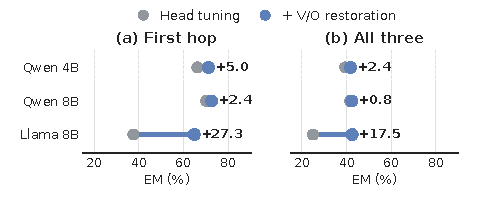
\includegraphics[width=.60\textwidth]{figures/data_main_restoration_revision.pdf}
\caption{\textbf{Restoring native prefill projections recovers constituent and joint answering.} The same tuned checkpoint is evaluated with and without its fixed restoration scope; three-run means.}
\label{fig:story_restoration}
\end{figure}
\begin{figure}[!ht]
\centering
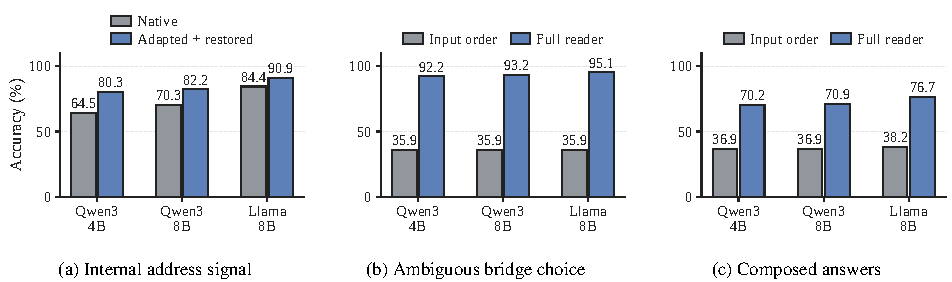
\includegraphics[width=.94\textwidth]{figures/data_main_repair_chain_revision.pdf}
\caption{\textbf{Address readout and evidence selection.} The full three-panel view complements the compact main-text comparison, retaining composed EM on ambiguous inputs.}
\label{fig:repair_closure_full}
\end{figure}
\textbf{Reproduction.} The paired routing analysis is implemented in \texttt{analysis/derive\_story\_adapted\_routing.py}; the four-state relation capture and aggregation use \texttt{capture\_paired\_relation\_reading.py} and \texttt{derive\_story\_relation\_reading.py} in the same directory. The archived per-head data, receiver-level records, aggregate CSVs and input hashes are retained in \texttt{analysis/figure\_data/}. Main-text figures are generated by the single numerical plotting entry point, \texttt{analysis/plot\_results.py}.
\FloatBarrier
